\documentclass{article}
\usepackage[pdftex,active,tightpage]{preview}
\setlength\PreviewBorder{2mm}
\usepackage{tikz}
\usetikzlibrary{patterns,snakes,shapes, calc}
\usetikzlibrary{decorations.pathreplacing}
\tikzstyle{clf}=[draw,outer sep=0pt, rounded rectangle, minimum height=0.8cm,
                 align=center]

\def \leveldist {-1.9}

\begin{document}
\begin{preview}
\begin{tikzpicture}
    \node[clf] (root)   at ( 0, 0) {$C_0$};

    % level 1
    \node[clf] (ped)    at (-5.0,1*\leveldist) {pedestrian};
    \node[clf] (wheel4) at (-3.0,1*\leveldist) {four$^+$-\\wheelers};
    \node[clf] (sign)   at (-1.0,1*\leveldist) {traffic\\sign};
    \node[clf] (wheel2) at ( 1.0,1*\leveldist) {two-\\wheelers};
    \node[inner sep=0pt] (street) at (3.0,1*\leveldist) {
\includegraphics[height=0.8cm]{road.jpg}};
    \node[inner sep=0pt] (other) at ( 5.0,1*\leveldist) {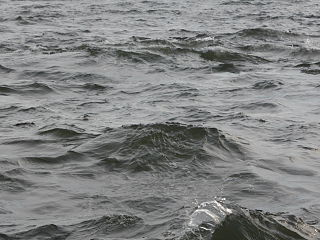
\includegraphics[height=0.8cm]{water.jpg}};
    \draw (root) -- (ped);
    \draw (root) -- (wheel4);
    \draw (root) -- (sign);
    \draw (root) -- (wheel2);
    \draw (root) -- (other);
    \draw (root) -- (street);

    % level 2
    \node[inner sep=0pt] (child) at (-5.3,1.7*\leveldist) {
\includegraphics[width=0.5cm]{child.jpg}};
    \node[inner sep=0pt] (adult) at (-4.6,1.6*\leveldist) {
\includegraphics[width=0.5cm]{adult.jpg}};
    \node[clf] (limit)      at (-2.0,2*\leveldist) {speed\\limit};
    \node[clf] (danger)     at (-0.5,2*\leveldist) {danger};
    \node[clf] (other)      at ( 0.8,2*\leveldist) {other};
    \node[inner sep=0pt] (bike)       at (0.5,1.5*\leveldist) {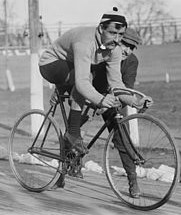
\includegraphics[height=0.6cm]{bike.jpg}};
    \node[inner sep=0pt] (motorcycle) at (1.3,1.5*\leveldist) {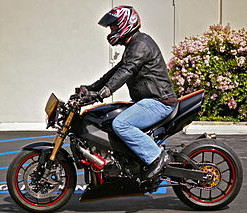
\includegraphics[height=0.6cm]{motorcycle.jpg}};
    \node[inner sep=0pt] (car) at (-3.5,1.5*\leveldist) {
\includegraphics[height=0.6cm]{car.jpg}};
    \node[inner sep=0pt] (lkw) at (-2.5,1.5*\leveldist) {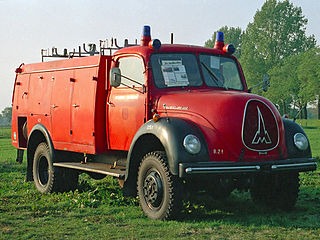
\includegraphics[height=0.6cm]{lkw.jpg}};
    \draw (sign) -- (limit);
    \draw (sign) -- (danger);
    \draw (sign) -- (other);
    \draw (wheel2) -- (bike);
    \draw (wheel2) -- (motorcycle);
    \draw (wheel4) -- (car);
    \draw (wheel4) -- (lkw);
    \draw (ped) -- (adult);
    \draw (ped) -- (child);

    % level 3
    \node[draw=red, text=black, line width=1.5pt, outer sep=1.5pt, circle,inner sep=0pt,minimum height=0.4cm] (speed30)  at (-2.3,2.5*\leveldist) {\tiny 30};
    \node[draw=red, text=black, line width=1.5pt, outer sep=1.5pt, circle,inner sep=0pt,minimum height=0.4cm] (speed80)  at (-1.7,2.5*\leveldist) {\tiny 80};
    \node[draw=red, text=black, line width=1.5pt, outer sep=1.5pt, circle,inner sep=0pt,minimum height=0.4cm] (speed120) at (-2.0,2.8*\leveldist) {\tiny 120};

    \node[inner sep=0pt] (dangera) at (-0.8,2.5*\leveldist) {
\includegraphics[width=0.5cm]{danger.png}};
    \node[inner sep=0pt] (dangerb) at (-0.2,2.5*\leveldist) {
\includegraphics[width=0.5cm]{danger-right.png}};
    \node[inner sep=0pt] (dangerc) at (-0.5,2.8*\leveldist) {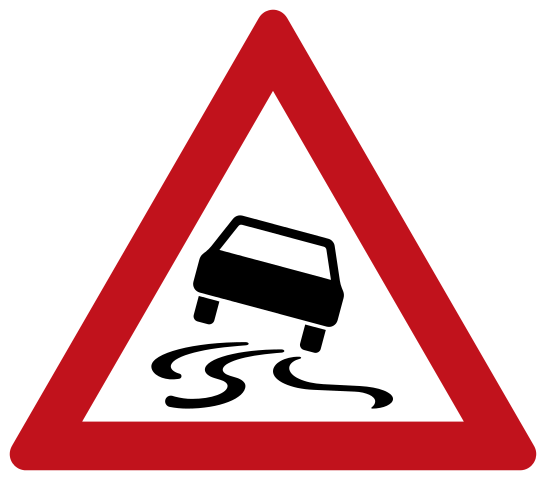
\includegraphics[width=0.5cm]{slippery.png}};

    \node[inner sep=0pt] (bikea) at (0.5,2.5*\leveldist) {
\includegraphics[width=0.5cm]{bike-sign.png}};
    \node[inner sep=0pt] (bikeb) at (1.1,2.5*\leveldist) {
\includegraphics[width=0.5cm]{bike-sign-french.png}};
    \node[inner sep=0pt] (bikec) at (0.8,2.8*\leveldist) {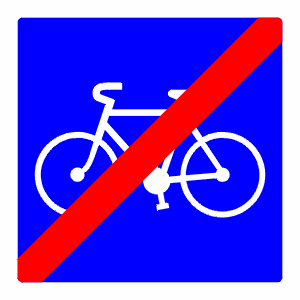
\includegraphics[width=0.5cm]{bike-sign-ove.png}};

    \draw (limit) -- (speed30);
    \draw (limit) -- (speed80);
    \draw (limit) -- (speed120);

    \draw (danger) -- (dangera);
    \draw (danger) -- (dangerb);
    \draw (danger) -- (dangerc);

    \draw (other) -- (bikea);
    \draw (other) -- (bikeb);
    \draw (other) -- (bikec);

\end{tikzpicture}
\end{preview}
\end{document}
